\pdfoutput=1
\RequirePackage[l2tabu, orthodox]{nag}


\documentclass{standalone}

 %\usepackage[notref,notcite]{showkeys} % USED TO SHOW EQUATION LABELS. REMOVE BEFORE FINAL VERSION

% \usepackage[pdftex]{hyperref}

\usepackage{lmodern}
\usepackage[T1]{fontenc}
\usepackage[utf8]{inputenc}
% \usepackage[english]{babel}
\usepackage{microtype} %Better font spacing

\usepackage{amsmath,amssymb,amsthm,mathrsfs,latexsym,mathtools,mathdots,booktabs,enumerate,tikz,bm,url,comment}
\usepackage[enableskew,vcentermath]{youngtab}
\usepackage[centertableaux]{ytableau}

\usetikzlibrary{arrows,positioning}
\usepackage[capitalize,noabbrev]{cleveref}


\definecolor{pBlue}{RGB}{86,139,190}
\definecolor{pCyan}{RGB}{149,186,201}
\definecolor{pSand}{RGB}{184,166,121}
\definecolor{pAlgae}{RGB}{87,115,135}
\definecolor{pSkin}{RGB}{236,216,167}
\definecolor{pGray}{RGB}{156,175,156}
\definecolor{pPink}{RGB}{215,114,127}
\definecolor{pOrange}{RGB}{211,153,80}



\begin{document}

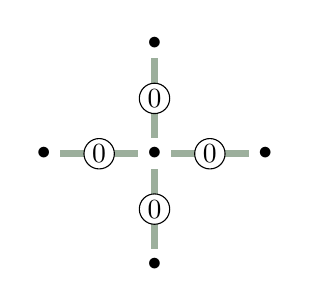
\begin{tikzpicture}[x=2em,y=2em,scale=1.0,circ/.style={circle,draw,inner sep=1pt, minimum width=0.8em}]
\draw[line width=2.5\pgflinewidth,pGray] (-2,0)--(2,0);
\draw[line width=2.5\pgflinewidth,pGray] (0,-2)--(0,2);
\node[circ,fill=white] at (-1, 0) {$0$};
\node[circ,fill=white] at ( 1, 0) {$0$};
\node[circ,fill=white] at ( 0,-1) {$0$};
\node[circ,fill=white] at ( 0, 1) {$0$};
\node[fill=white] at ( 0, 0) {$\bullet$};
\node[fill=white] at (-2, 0) {$\bullet$};
\node[fill=white] at ( 2, 0) {$\bullet$};
\node[fill=white] at ( 0,-2) {$\bullet$};
\node[fill=white] at ( 0, 2) {$\bullet$};
\end{tikzpicture}


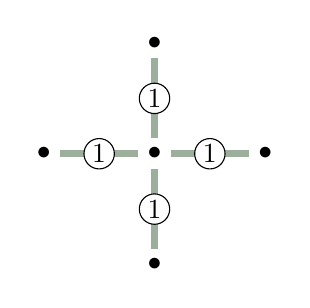
\begin{tikzpicture}[x=2em,y=2em,scale=1.0,circ/.style={circle,draw,inner sep=1pt, minimum width=0.8em}]
\draw[line width=2.5\pgflinewidth,pGray] (-2,0)--(2,0);
\draw[line width=2.5\pgflinewidth,pGray] (0,-2)--(0,2);
\node[circ,fill=white] at (-1, 0) {$1$};
\node[circ,fill=white] at ( 1, 0) {$1$};
\node[circ,fill=white] at ( 0,-1) {$1$};
\node[circ,fill=white] at ( 0, 1) {$1$};
\node[fill=white] at ( 0, 0) {$\bullet$};
\node[fill=white] at (-2, 0) {$\bullet$};
\node[fill=white] at ( 2, 0) {$\bullet$};
\node[fill=white] at ( 0,-2) {$\bullet$};
\node[fill=white] at ( 0, 2) {$\bullet$};
\end{tikzpicture}



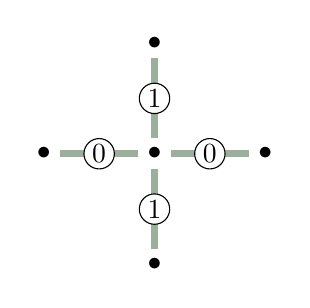
\begin{tikzpicture}[x=2em,y=2em,scale=1.0,circ/.style={circle,draw,inner sep=1pt, minimum width=0.8em}]
\draw[line width=2.5\pgflinewidth,pGray] (-2,0)--(2,0);
\draw[line width=2.5\pgflinewidth,pGray] (0,-2)--(0,2);
\node[circ,fill=white] at (-1, 0) {$0$};
\node[circ,fill=white] at ( 1, 0) {$0$};
\node[circ,fill=white] at ( 0,-1) {$1$};
\node[circ,fill=white] at ( 0, 1) {$1$};
\node[fill=white] at ( 0, 0) {$\bullet$};
\node[fill=white] at (-2, 0) {$\bullet$};
\node[fill=white] at ( 2, 0) {$\bullet$};
\node[fill=white] at ( 0,-2) {$\bullet$};
\node[fill=white] at ( 0, 2) {$\bullet$};
\end{tikzpicture}


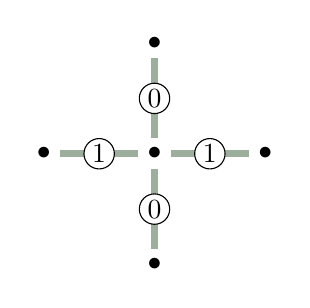
\begin{tikzpicture}[x=2em,y=2em,scale=1.0,circ/.style={circle,draw,inner sep=1pt, minimum width=0.8em}]
\draw[line width=2.5\pgflinewidth,pGray] (-2,0)--(2,0);
\draw[line width=2.5\pgflinewidth,pGray] (0,-2)--(0,2);
\node[circ,fill=white] at (-1, 0) {$1$};
\node[circ,fill=white] at ( 1, 0) {$1$};
\node[circ,fill=white] at ( 0,-1) {$0$};
\node[circ,fill=white] at ( 0, 1) {$0$};
\node[fill=white] at ( 0, 0) {$\bullet$};
\node[fill=white] at (-2, 0) {$\bullet$};
\node[fill=white] at ( 2, 0) {$\bullet$};
\node[fill=white] at ( 0,-2) {$\bullet$};
\node[fill=white] at ( 0, 2) {$\bullet$};
\end{tikzpicture}


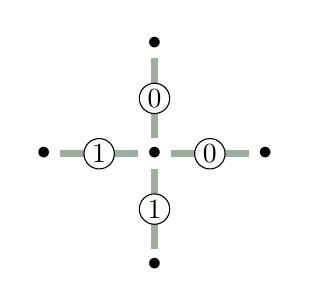
\begin{tikzpicture}[x=2em,y=2em,scale=1.0,circ/.style={circle,draw,inner sep=1pt, minimum width=0.8em}]
\draw[line width=2.5\pgflinewidth,pGray] (-2,0)--(2,0);
\draw[line width=2.5\pgflinewidth,pGray] (0,-2)--(0,2);
\node[circ,fill=white] at (-1, 0) {$1$};
\node[circ,fill=white] at ( 1, 0) {$0$};
\node[circ,fill=white] at ( 0,-1) {$1$};
\node[circ,fill=white] at ( 0, 1) {$0$};
\node[fill=white] at ( 0, 0) {$\bullet$};
\node[fill=white] at (-2, 0) {$\bullet$};
\node[fill=white] at ( 2, 0) {$\bullet$};
\node[fill=white] at ( 0,-2) {$\bullet$};
\node[fill=white] at ( 0, 2) {$\bullet$};
\end{tikzpicture}

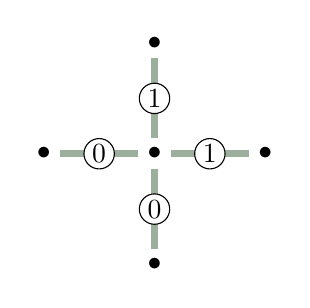
\begin{tikzpicture}[x=2em,y=2em,scale=1.0,circ/.style={circle,draw,inner sep=1pt, minimum width=0.8em}]
\draw[line width=2.5\pgflinewidth,pGray] (-2,0)--(2,0);
\draw[line width=2.5\pgflinewidth,pGray] (0,-2)--(0,2);
\node[circ,fill=white] at (-1, 0) {$0$};
\node[circ,fill=white] at ( 1, 0) {$1$};
\node[circ,fill=white] at ( 0,-1) {$0$};
\node[circ,fill=white] at ( 0, 1) {$1$};
\node[fill=white] at ( 0, 0) {$\bullet$};
\node[fill=white] at (-2, 0) {$\bullet$};
\node[fill=white] at ( 2, 0) {$\bullet$};
\node[fill=white] at ( 0,-2) {$\bullet$};
\node[fill=white] at ( 0, 2) {$\bullet$};
\end{tikzpicture}

\end{document}

